\documentclass{beamer}
\usepackage{booktabs}
\usepackage{amsmath}
%%\usepackage{blkarray}
\mode<presentation>
{
%  \usetheme{Malmoe}
\usetheme{default}
%\usecolortheme{seahorse}
  % or ...

 \setbeamercovered{transparent}
  % or whatever (possibly just delete it)
 \setbeamertemplate{footline}[default]
 \setbeamertemplate{navigation symbols}{\insertslidenavigationsymbol\insertframenavigationsymbol\insertdocnavigationsymbol}
}
\usepackage[english]{babel}

\title{What can your library do for you?}
\author{Rajarshi Guha, Dac-Trung Nguyen, Ajit Jadhav\\
NIH NCATS}

\begin{document}

\begin{frame}
  \titlepage
\end{frame}

\begin{frame}
  \frametitle{Library Design}
  \begin{itemize}
  \item Historical collections and assay data provide information on how a set of compounds has faired
  \item Use (dis)similarity and machine learning to construct new collections that show similar behavior
    \begin{itemize}
    \item Plus various constraints
    \end{itemize}
  \item If sufficiently annotated, compound behavior can be correlated to assay and biology characteristics
  \end{itemize}
\end{frame}

\begin{frame}
  \frametitle{Two Questions}
  How likely are compounds, associated with a  given annotation, identified as active?
  \vskip 2em
  Given a new set of compounds, what sets of assay conditions (as implied by the annotations) will they be active in? 
\end{frame}

\begin{frame}
  \frametitle{Prior Work}
  \begin{itemize}
  \item BAO annotated datasets
    \begin{itemize}
    \item \href{http://www.ncbi.nlm.nih.gov/pubmed/24441647}{de Souza et al, 2014}; \href{http://www.ncbi.nlm.nih.gov/pubmed/23155465}{Vempati et al, 2012}
    \end{itemize}
  \item Analyzing HTS datasets using BAO
    \begin{itemize}
    \item \href{http://www.ncbi.nlm.nih.gov/pubmed/25512330}{Zander-Balderud et al, 2015}; \href{http://www.ncbi.nlm.nih.gov/pubmed/21471461}{Sch\"{u}rer et al, 2011}
    \end{itemize}
  \item Semi-automated annotation of assay descriptions using the BAO 
    \begin{itemize}
    \item \href{http://www.ncbi.nlm.nih.gov/pubmed/25165633}{Clark et al, 2014}
    \end{itemize}
  \end{itemize}
\end{frame}

\begin{frame}
  \frametitle{BAO 2.0}
  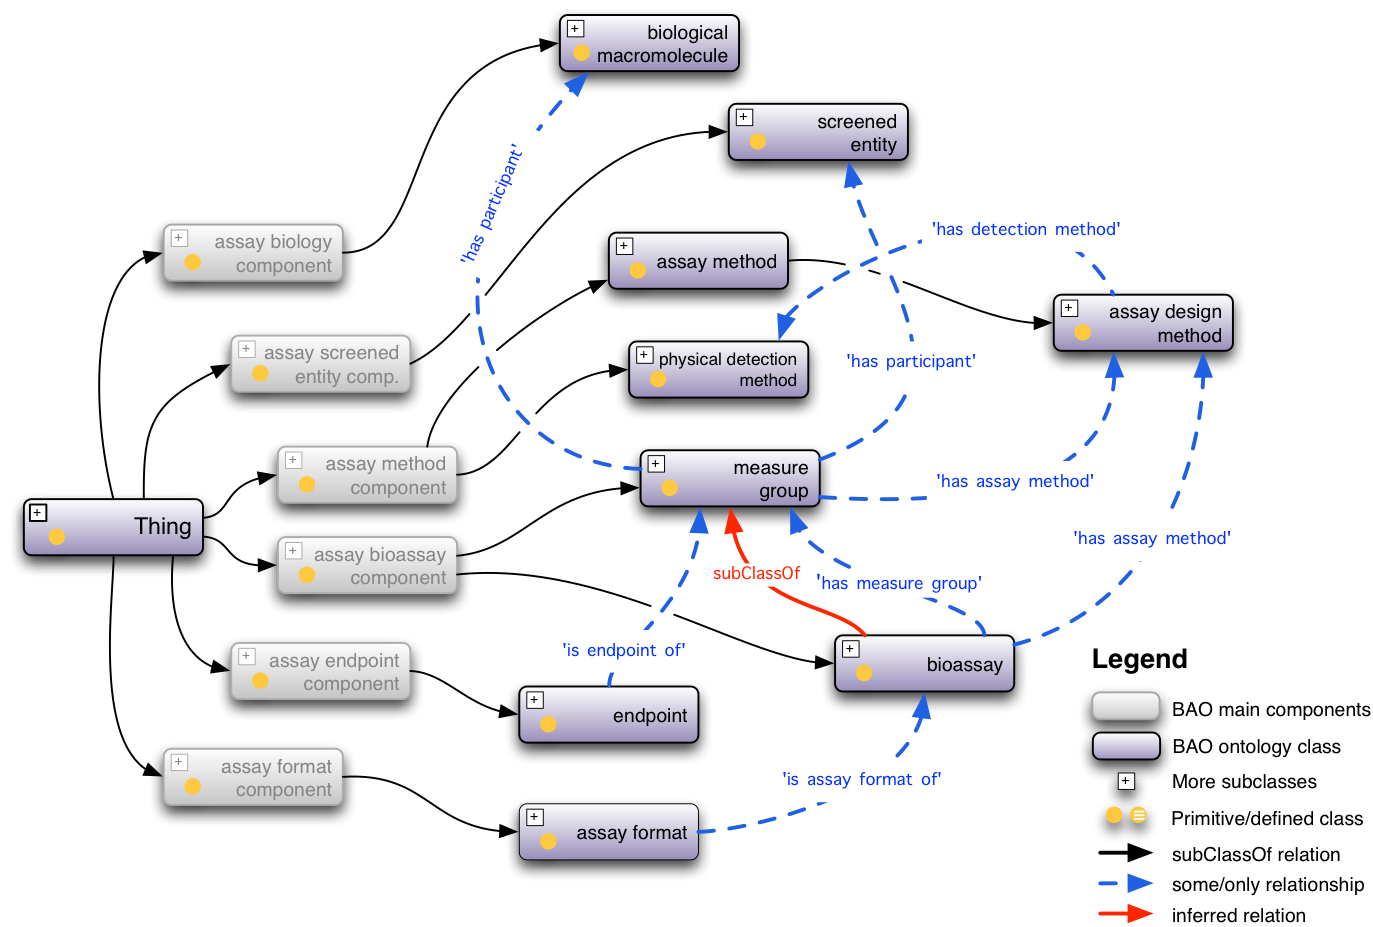
\includegraphics[height=3.0in]{bao}
\end{frame}

\begin{frame}
  \frametitle{Assay Modeling}
  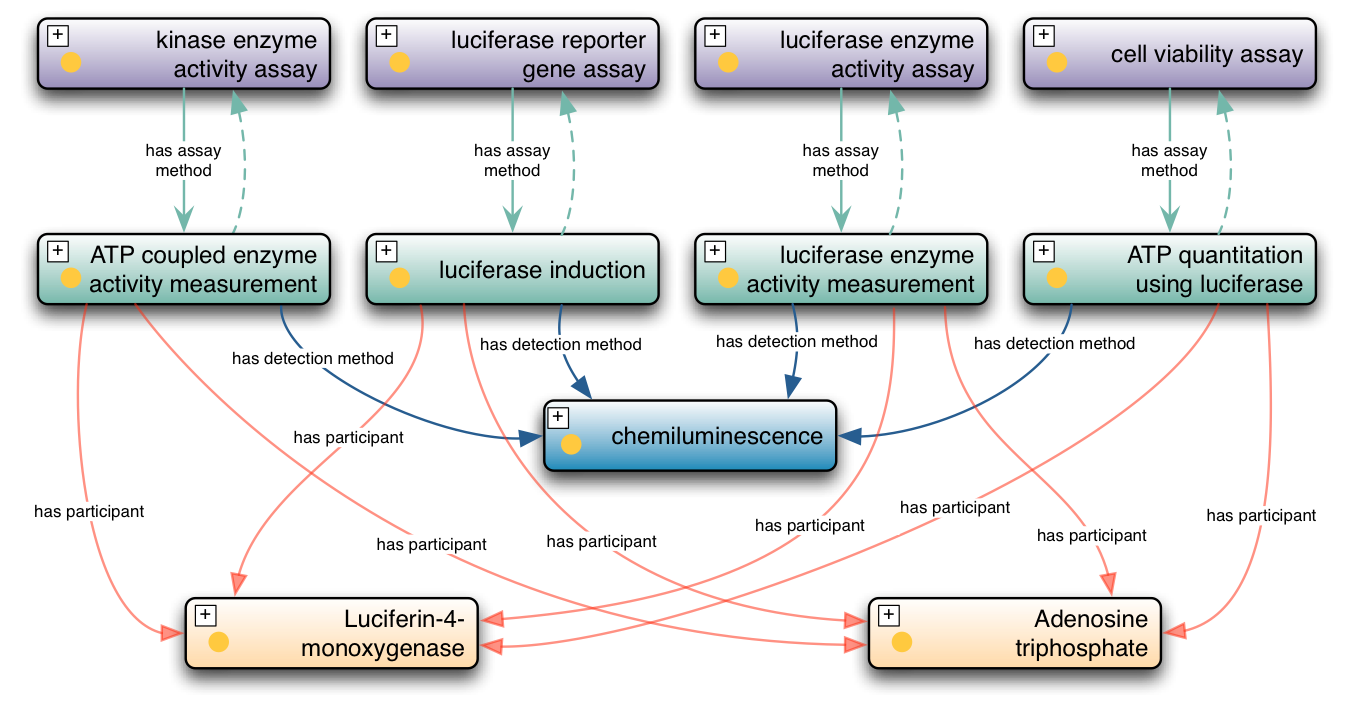
\includegraphics[height=3.0in]{assaymodel}
\end{frame}

\end{document}
